\documentclass[
]{jss}

%% recommended packages
\usepackage{orcidlink,thumbpdf,lmodern}

\usepackage[utf8]{inputenc}

\author{
Hanne Oberman\\Utrecht University \And Johanna Munoz Avila\\University
Medical Center Utrecht \AND Valentijn de Jong\\University Medical
Center Utrecht \And Gerko Vink\\Utrecht University \AND Thomas
Debray\\University Medical Center Utrecht
}
\title{Imputation of Incomplete Multilevel Data with \pkg{mice}}

\Plainauthor{Hanne Oberman, Johanna Munoz Avila, Valentijn de
Jong, Gerko Vink, Thomas Debray}
\Plaintitle{Imputation of Incomplete Multilevel Data with mice}
\Shorttitle{Multilevel \pkg{mice}}


\Abstract{
This is a tutorial paper on imputing incomplete multilevel data with
\pkg{mice}. Footnotes in the current version show work in progress/under
construction. The last section is not part of the manuscript, but purely
for reminders. We aim to submit at JSS, so there is no word count limit
(``There is no page limit, nor a limit on the number of figures or
tables''). {[}Just adding some text to get a better guess of what the
actura abstract will look like: Lorem ipsum dolor sit amet, consectetur
adipiscing elit, sed do eiusmod tempor incididunt ut labore et dolore
magna aliqua. Ut enim ad minim veniam, quis nostrud exercitation ullamco
laboris nisi ut aliquip ex ea commodo consequat. Duis aute irure dolor
in reprehenderit in voluptate velit esse cillum dolore eu fugiat nulla
pariatur. Excepteur sint occaecat cupidatat non proident, sunt in culpa
qui officia deserunt mollit anim id est laborum.{]}
}

\Keywords{missing
data, multilevel, clustering, \pkg{mice}, \proglang{R}}
\Plainkeywords{missing data, multilevel, clustering, mice, R}

%% publication information
%% \Volume{50}
%% \Issue{9}
%% \Month{June}
%% \Year{2012}
%% \Submitdate{}
%% \Acceptdate{2012-06-04}

\Address{
    Hanne Oberman\\
    Utrecht University\\
    Padualaan 14\\
3584 CH Utrecht\\
  E-mail: \email{h.i.oberman@uu.nl}\\
  URL: \url{https://hanneoberman.github.io/}\\~\\
          }


% tightlist command for lists without linebreak
\providecommand{\tightlist}{%
  \setlength{\itemsep}{0pt}\setlength{\parskip}{0pt}}



\usepackage{graphicx}
\usepackage{mathtools}
\usepackage{ulem}

\usepackage{amsmath}

\begin{document}



\hypertarget{introduction}{%
\section{Introduction}\label{introduction}}

In many contemporary data analysis efforts, some form of hierarchical or
clustered data structures are recorded. In the simplest case, such a
structure entails the nesting of units within clusters (e.g., students
within school classes). More complex clustered structures may occur when
there are multiple hierarchical levels (e.g., patients within hospitals
within regions or countries), or when the clustering is non-nested
(e.g., electronic health record data from diverse settings and
populations within large databases). The clustered structure of
multilevel data should be taken into account when developing analysis
models: 1) for the simple reason that groups of observations share some
common variance, and 2) because ignoring multilevel structures can be
harmful to the statistical inferences and introduce bias in estimators
\citep{hox17}. There are many names for models that take clustering into
account. Some popular examples are `multilevel models', `hierarchical
models', `mixed effect models' and `random effect models'. Table
\ref{tab:clus} provides an overview of some key concepts in multilevel
modeling.

\begin{table}[tb]
\caption{Concepts in multilevel methods}
\label{tab:clus}
\centering
\begin{tabular}{ll}
\hline
\textbf{Concept} & \textbf{Details}   \\
\hline
ICC                 & The variability due to clustering is often measured by means of the \\
                    & intraclass coefficient (ICC). The ICC can be seen as the percentage \\
                    & of variance that can be attributed to the cluster-level, where a high \\
                    & ICC would indicate that a lot of variability is due to the cluster \\
                    & structure. \\
Random effect       & Multilevel models typically accommodate for variability by including \\
                    & a separate group mean for each cluster. In addition to random \\
                    & intercepts, multilevel models can also include random effects and \\
                    & heterogeneous residual error variances across clusters [see e.g. \\
                    & @gelm06, @hox17 and @jong21]. TODO: add stratification. \\
\hline
\end{tabular}
\end{table}

\hypertarget{missingness-in-multilevel-data}{%
\subsection{Missingness in multilevel
data}\label{missingness-in-multilevel-data}}

The process of analyzing multilevel data is further complicated when not
all data entries are observed. Just as with single level data,
missingness may occur at the unit level. But with multiple levels of
data comes the potential for clustered missingness. Therefore,
incomplete multilevel data can be categorized into two general patterns:
systematic missingness and sporadic missingness \citep{resc13}.
Systematic missingness implies that one or more variables are never
observed in a certain cluster. With sporadic missingness there may be
observed data for some but not all units in a cluster
\citep{buur18, jola18}. We have visualized this difference in Figure 1,
which shows an \(n \times p\) set \(\mathbf{X} = X_1, \dots, X_p\), with
\(n\) units distributed over \(N\) clusters and \(p\) variables.

\begin{CodeChunk}
\begin{figure}

{\centering 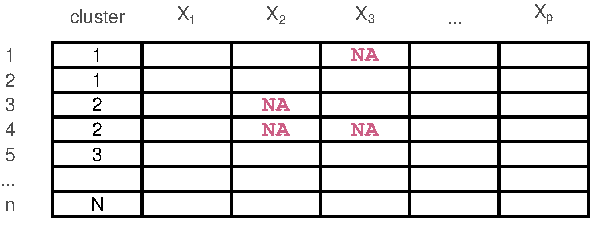
\includegraphics{Imputation_of_Incomplete_Multilevel_Data_files/figure-latex/patterns-1} 

}

\caption[Missingness in multilevel data]{Missingness in multilevel data}\label{fig:patterns}
\end{figure}
\end{CodeChunk}

Column \(X_1\) in Figure 1 is completely observed, column \(X_2\) is
systematically missing in cluster 2, and column \(X_3\) is sporadically
missing. To analyze these incomplete data, we have to take the nature of
the missingness and the cluster structure into account. For example, the
sporadic missingness in \(X_3\) could be easily amended if this would be
a cluster-level variable (and thus constant within clusters). We could
then just extrapolate the true (but missing) value of \(X_3\) for unit 1
from unit 2, and the value for unit 4 from unit 3. If \(X_3\) would
instead be a unit-level variable (which may vary within clusters), we
could not just recover the unobserved `truth', but would need to use
some kind of missing data method, or discard the incomplete units
altogether (i.e., complete case analysis). Complete case analysis can
however introduce bias in statistical inferences and lowers statistical
power. Further, with the systematic missingness in \(X_2\), it would be
impossible to fit a multilevel model without accommodating the
missingness in some way. Complete case analysis in that case would mean
excluding the entire cluster from the analyses. The wrong choice of
missing data handling method can thus be extremely harmful to the
inferences.

A key characteristic of the missing data to take into account in
analyses is the mechanism behind the missingness. We distinguish between
MCAR, MAR and MNAR in theory (see Table \ref{tab:miss}), but in practice
this distinction is less clear. Since the essence of the true
non-response mechanism may not be known, it is generally inferred or
assumed to be ignorable (i.e., MCAR or MAR). {[}TODO: add that this
assumption may not always be valid, especially with modern types of big
dasta sources.{]} Depending on the actual missingness-generating
mechanism, missing data handling strategies may be more or less
suitable, see e.g., \citet{yuce08} and \citet{hox15}.

\begin{table}[tb]
\caption{Concepts in missing data methods}
\label{tab:miss}
\centering
\begin{tabular}{ll}
\hline
\textbf{Concept} & \textbf{Details}   \\
\hline
MCAR    & Missing Completely At Random, where the probability to be missing is equal \\
& across all data entries \\
MAR     & Missing At Random, where the probability to be missing depends on observed \\
& information \\
MNAR    & Missing Not At Random (MNAR), where the probability to be missing \\
& depends on unrecorded information, making the missingness non-ignorable \\
& [@rubi76; @meng94]. \\
& [TODO: add congeniality, but maybe in-text?] \\
\hline
\end{tabular}
\end{table}

Since excluding observations is not a desirable workflow, the
missingness in multilevel data should be accommodated \emph{before} or
\emph{within} the analysis of scientific interest. In this paper, we
focus on the former approach: imputing (i.e., filling in) the missing
data with plausible values, whereafter the completed data may be
analyzed as if it were completely observed. Imputation separates the
missing data problem from the scientific problem, which makes the
missing data strategy very generic and popular. If each missing value is
replaced multiple times, the resulting inferences may validly convey the
uncertainty due to missingness \citep[c.f.][]{rubi76}. The \proglang{R}
package \pkg{mice} has become the de-facto standard for imputation by
chained equations, which iteratively solves the missingness on a
variable-by-variable basis. \pkg{mice} is known to yield valid
inferences under many different missing data circumstances
\citep{buur18}. In this paper, we will discuss how to use \pkg{mice} in
the context of multilevel data.

{[}TODO: clarify why clustering is relevant during imputation, and why
this exposes the need for specialized imputation methods and more
attention during their implementation (``thou shall not simply run
\texttt{mice()} on any incomplete dataset''). And add overview of
possible predictor matrix values.{]}

\hypertarget{aim-of-this-paper}{%
\subsection{Aim of this paper}\label{aim-of-this-paper}}

This papers serves as a tutorial for imputing incomplete multilevel data
with \pkg{mice} in \proglang{R}. We provide practical guidelines and
code snippets for different missing data situations, including
non-ignorable mechanisms. For reasons of brevity, we focus on multilevel
imputation by chained equations with \pkg{mice} exclusively; other
imputation methods and packages (e.g., \pkg{jomo} and \pkg{mdmb}) are
outside the scope of this tutorial. Assumed knowledge includes basic
familiarity with multilevel imputation \citep[see e.g.][ and
\citet{grun18}]{audi18} and the \pkg{lme4} notation for multilevel
models (see Table \ref{tab:mod}).

\begin{table}[tb]
\caption{Notation}
\label{tab:mod}
\centering
\begin{tabular}{ll}
\hline
\textbf{Concept} & \textbf{Details}   \\
\hline
& [TODO: explain \pkg{lme4} notation here] \\
\hline
\end{tabular}
\end{table}

TODO: add paragraph about novice and more experienced readers.

\hypertarget{case-study}{%
\section{Case study}\label{case-study}}

We illustrate how to impute incomplete multilevel data by means of a
case study: \texttt{impact} from the \pkg{metamisc} package
\citep[empirical data on traumatic brain injuries, \(n = 11,022\) units
across \(N = 15\) clusters,][]{metamisc}. {[}TODO: add more info about
the complete data.{]} The \texttt{impact} data set contains traumatic
brain injury data on \(n = 11022\) patients clustered in \(N = 15\)
studies with the following 11 variables:

\begin{itemize}
\tightlist
\item
  \texttt{name} Name of the study,
\item
  \texttt{type} Type of study (RCT: randomized controlled trial, OBS:
  observational cohort),
\item
  \texttt{age} Age of the patient,
\item
  \texttt{motor\_score} Glasgow Coma Scale motor score,
\item
  \texttt{pupil} Pupillary reactivity,
\item
  \texttt{ct} Marshall Computerized Tomography classification,
\item
  \texttt{hypox} Hypoxia (0=no, 1=yes),
\item
  \texttt{hypots} Hypotension (0=no, 1=yes),
\item
  \texttt{tsah} Traumatic subarachnoid hemorrhage (0=no, 1=yes),
\item
  \texttt{edh} Epidural hematoma (0=no, 1=yes),
\item
  \texttt{mort} 6-month mortality (0=alive, 1=dead).
\end{itemize}

The analysis model for this dataset is a prediction model with
\texttt{mort} as the outcome. In this tutorial we'll estimate the
adjusted prognostic effect of \texttt{ct} on unfortunate outcomes. The
estimand is the adjusted odds ratio for \texttt{ct}, after including
\texttt{type}, \texttt{age} \texttt{motor\_score} and \texttt{pupil}
into the analysis model:

\begin{CodeChunk}
\begin{CodeInput}
R> mod <- mort ~ 1 + type + age + motor_score + pupil + ct + (1 | name) # TODO: add random effects ct?
\end{CodeInput}
\end{CodeChunk}

Note that variables \texttt{hypots}, \texttt{hypox}, \texttt{tsah} and
\texttt{edh} are not part of the analysis model, and may thus serve as
auxiliary variables for imputation.

\hypertarget{setup}{%
\subsection{Setup}\label{setup}}

{[}TODO: Add environment info, seed and version number(s) somewhere.{]}
Set up the R environment and load the necessary packages:

\begin{CodeChunk}
\begin{CodeInput}
R> set.seed(2022)
R> library(mice)         # for imputation
R> library(ggmice)       # for visualization
R> library(ggplot2)      # for visualization
R> library(dplyr)        # for data wrangling
R> library(lme4)         # for multilevel modeling
R> library(broom.mixed)  # for multilevel estimates
R> library(mitml)        # for multilevel pooling
\end{CodeInput}
\end{CodeChunk}

The \texttt{impact} data included in the \pkg{metamisc} package is a
complete data set. The original data has already been imputed once
(Steyerberg et al, 2008). For the purpose of this tutorial we have
induced missingness (mimicking the missing data in the original data set
before imputation). The resulting incomplete data can be accessed from
\href{https://zenodo.com}{zenodo link to be created}. TODO: email script
to thomas.

Load the complete and incomplete data into the R workspace:

\begin{CodeChunk}
\begin{CodeInput}
R> data("impact", package = "metamisc")      # complete data
R> dat <- read.table("link/to/the/data.txt") # incomplete data
\end{CodeInput}
\end{CodeChunk}

We will use the following estimates as comparative truth in this
tutorial {[}TODO: make this a table or forest plot instead, to see if
there is heterogeneity in the association of \texttt{ct} with
\texttt{mort}{]}:

\begin{CodeChunk}
\begin{CodeInput}
R> fit <- glmer(mod, family = "binomial", data = impact) # fit the model
R> tidy(fit, conf.int = TRUE, exponentiate = TRUE)       # print estimates
\end{CodeInput}
\begin{CodeOutput}
# A tibble: 11 x 9
   effect group term  estimate std.error statistic    p.value conf.low conf.high
   <chr>  <chr> <chr>    <dbl>     <dbl>     <dbl>      <dbl>    <dbl>     <dbl>
 1 fixed  <NA>  (Int~    0.101   0.0173     -13.4   4.94e- 41   0.0723     0.141
 2 fixed  <NA>  type~    0.713   0.123       -1.96  5.01e-  2   0.509      1.00 
 3 fixed  <NA>  age      1.03    0.00165     20.2   2.13e- 90   1.03       1.04 
 4 fixed  <NA>  moto~    0.553   0.0386      -8.50  1.95e- 17   0.482      0.634
 5 fixed  <NA>  moto~    0.405   0.0289     -12.7   8.43e- 37   0.352      0.466
 6 fixed  <NA>  moto~    0.275   0.0202     -17.6   1.67e- 69   0.239      0.318
 7 fixed  <NA>  pupi~    3.73    0.230       21.4   2.09e-101   3.31       4.21 
 8 fixed  <NA>  pupi~    1.87    0.133        8.80  1.36e- 18   1.63       2.15 
 9 fixed  <NA>  ctIII    2.25    0.157       11.6   5.12e- 31   1.96       2.58 
10 fixed  <NA>  ctIV~    2.30    0.136       14.0   9.47e- 45   2.05       2.58 
11 ran_p~ name  sd__~    0.277  NA           NA    NA          NA         NA    
\end{CodeOutput}
\end{CodeChunk}

\begin{CodeChunk}


\begin{center}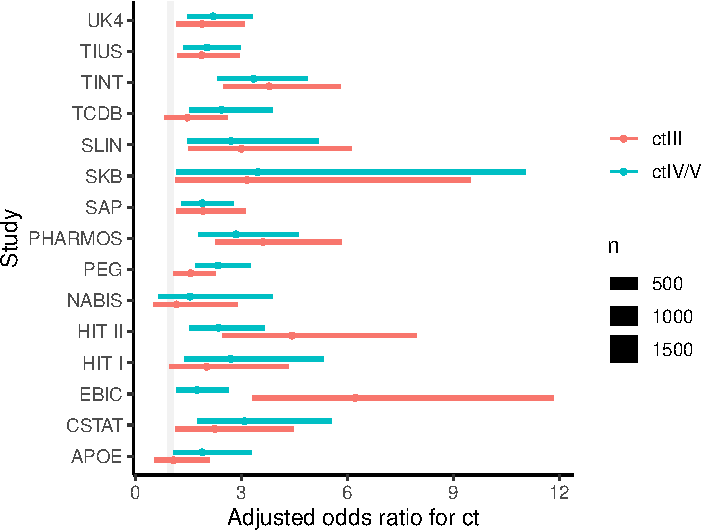
\includegraphics{Imputation_of_Incomplete_Multilevel_Data_files/figure-latex/forest-1} \end{center}

\end{CodeChunk}

{[}TODO: add ICC before/after imputation and interpret: This tells us
that the multilevel structure of the data should probably be taken into
account. If we don't, we'll may end up with incorrect imputations,
biasing the effect of the clusters towards zero.{]}

{[}TODO: add descriptive statistics of the complete and incomplete
data.{]}

\hypertarget{missingness}{%
\subsection{Missingness}\label{missingness}}

To explore the missingness, it is wise to look at the missing data
pattern:

\begin{CodeChunk}
\begin{CodeInput}
R> plot_pattern(dat, rotate = TRUE)  # plot missingness pattern
\end{CodeInput}


\begin{center}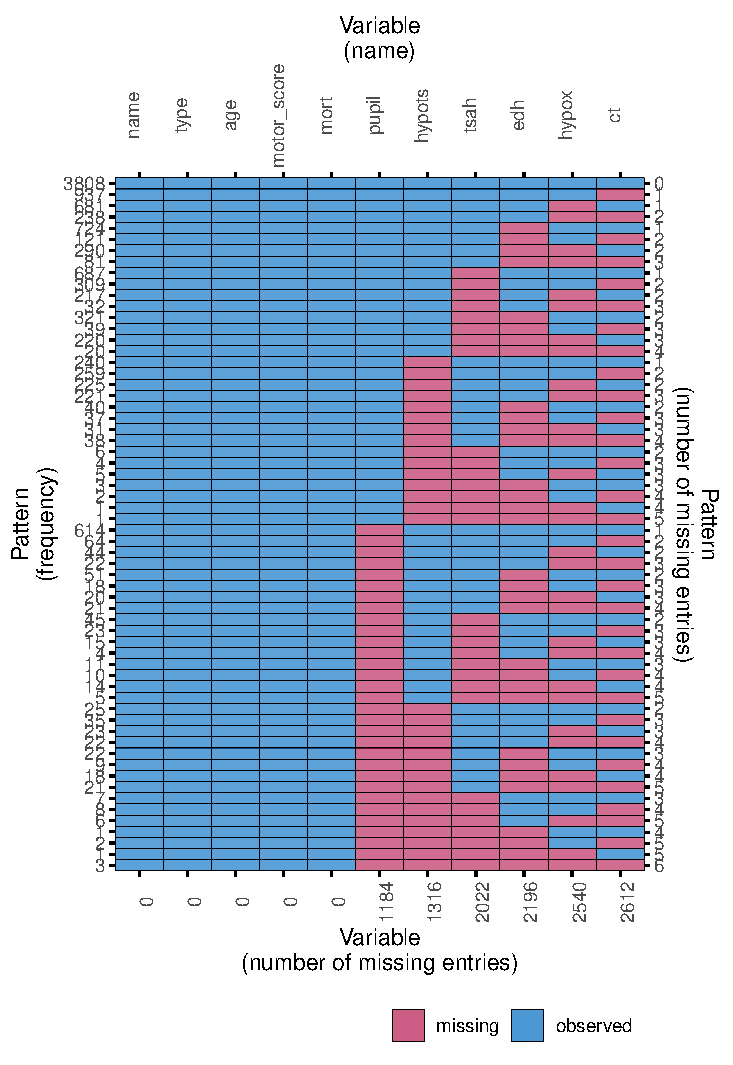
\includegraphics{Imputation_of_Incomplete_Multilevel_Data_files/figure-latex/pattern-1} \end{center}

\end{CodeChunk}

This shows\ldots{} {[}TODO: fill in that we need to impute \texttt{ct}
and \texttt{pupil}.{]} TODO: remove axis labels

To develop the best imputation model, we need to investigate the
relations between the observed values of the incomplete variables and
the observed values of other variables, and the relation between the
missingness indicators of the incomplete variables and the observed
values of the other variables. To see whether the missingness depends on
the observed values of other variables, we\ldots{} {[}TODO: fill in that
we can test this statistically or use visual inspection (e.g.~a
histogram faceted by the missingness indicator).{]}

We should impute the variables \texttt{ct} and \texttt{pupil} and any
auxiliary variables we might want to use to impute these incomplete
analysis model variables. We can evaluate which variables may be useful
auxiliaries by plotting the pairwise complete correlations:

\begin{CodeChunk}
\begin{CodeInput}
R> plot_corr(dat, rotate = TRUE) # plot correlations 
\end{CodeInput}


\begin{center}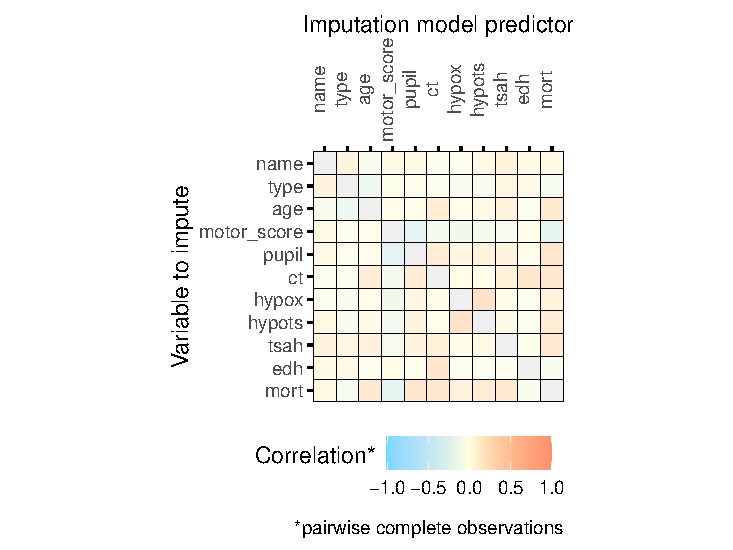
\includegraphics{Imputation_of_Incomplete_Multilevel_Data_files/figure-latex/impact_corr-1} \end{center}

\end{CodeChunk}

This shows us that \texttt{hypox} and \texttt{hypot} would not be useful
auxiliary variables for imputing \texttt{ct}. Depending on the minimum
required correlation, \texttt{tsah} could be useful, while \texttt{edh}
has the strongest correlation with \texttt{ct} out of all the variables
in the data and should definitely be included in the imputation model.
For the imputation of \texttt{pupil}, none of the potential auxiliary
variables has a very strong relation, but \texttt{hypots} could be used.
We conclude that we can exclude \texttt{hypox} from the data, since this
is neither an analysis model variable nor an auxiliary variable for
imputation:

\begin{CodeChunk}
\begin{CodeInput}
R> dat <- select(dat, !hypox)  # remove variable
\end{CodeInput}
\end{CodeChunk}

\hypertarget{complete-case-analysis}{%
\subsection{Complete case analysis}\label{complete-case-analysis}}

As previously stated, complete case analysis lowers statistical power
and may bias results. The complete case analysis estimates are:

\begin{CodeChunk}
\begin{CodeInput}
R> fit <- glmer(mod, family = "binomial", data = na.omit(dat)) # fit the model
R> tidy(fit, conf.int = TRUE, exponentiate = TRUE)             # print estimates
\end{CodeInput}
\begin{CodeOutput}
# A tibble: 11 x 9
   effect  group term  estimate std.error statistic   p.value conf.low conf.high
   <chr>   <chr> <chr>    <dbl>     <dbl>     <dbl>     <dbl>    <dbl>     <dbl>
 1 fixed   <NA>  (Int~   0.0863   0.0182     -11.6   2.99e-31   0.0571     0.130
 2 fixed   <NA>  type~   0.757    0.137       -1.54  1.22e- 1   0.531      1.08 
 3 fixed   <NA>  age     1.03     0.00265     12.9   7.40e-38   1.03       1.04 
 4 fixed   <NA>  moto~   0.651    0.0732      -3.82  1.34e- 4   0.522      0.811
 5 fixed   <NA>  moto~   0.489    0.0555      -6.30  2.97e-10   0.391      0.611
 6 fixed   <NA>  moto~   0.274    0.0321     -11.0   2.28e-28   0.218      0.345
 7 fixed   <NA>  pupi~   3.20     0.317       11.7   8.18e-32   2.63       3.88 
 8 fixed   <NA>  pupi~   1.75     0.195        5.06  4.27e- 7   1.41       2.18 
 9 fixed   <NA>  ctIII   2.41     0.268        7.89  3.05e-15   1.94       2.99 
10 fixed   <NA>  ctIV~   2.30     0.214        8.95  3.55e-19   1.92       2.76 
11 ran_pa~ name  sd__~   0.230   NA           NA    NA         NA         NA    
\end{CodeOutput}
\end{CodeChunk}

As we can see\ldots{} {[}TODO: fill in.{]}

\hypertarget{imputation-model}{%
\subsection{Imputation model}\label{imputation-model}}

The first imputation model that we'll use is likely to be invalid. We do
\emph{not} use the cluster identifier \texttt{name} as imputation model
predictor. With this model, we ignore the multilevel structure of the
data, despite the high ICC. This assumes exchangeability between units.
We include it purely to illustrate the effects of ignoring the
clustering in our imputation effort. We'll use the default imputation
methods in \texttt{mice()} (predictive mean matching to impute the
continuous variables and logistic regression to impute binary
variables).

\begin{center}\rule{0.5\linewidth}{0.5pt}\end{center}

\begin{center}

Updated until here!

\end{center}

\begin{center}\rule{0.5\linewidth}{0.5pt}\end{center}

Create a methods vector and predictor matrix, and make sure
\texttt{name} is not included as predictor:

\begin{CodeChunk}
\begin{CodeInput}
R> meth <- make.method(dat) # methods vector
R> pred <- quickpred(dat)   # predictor matrix
R> plot_pred(pred)
\end{CodeInput}


\begin{center}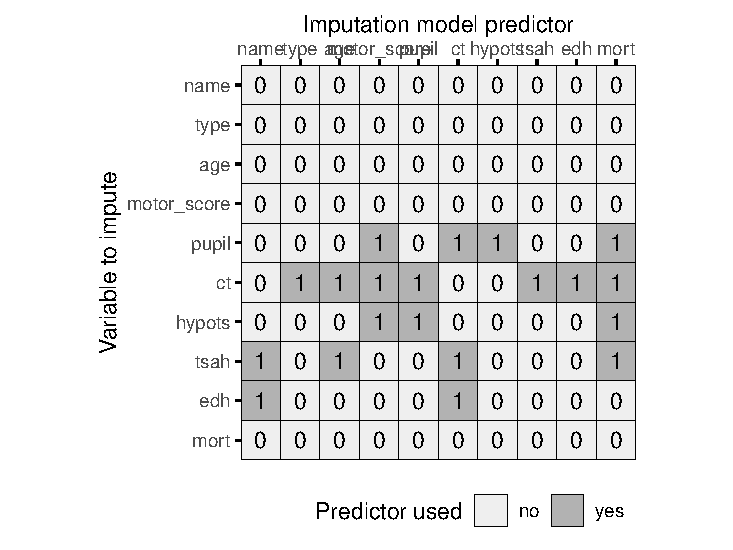
\includegraphics{Imputation_of_Incomplete_Multilevel_Data_files/figure-latex/ignore-1} \end{center}

\end{CodeChunk}

{[}TODO: mutate data to get the right data types for imputation
(e.g.~integer for clustering variable).{]}

\hypertarget{discussion}{%
\section{Discussion}\label{discussion}}

\begin{itemize}
\item
  JOMO in \pkg{mice} -\textgreater{} on the side for now
\item
  Additional levels of clustering
\item
  More complex data types: timeseries and polynomial relationship in the
  clustering.
\end{itemize}

\hypertarget{think-about}{%
\section{Think about}\label{think-about}}

\begin{itemize}
\item
  Adding some kind of help function to mice that suggests a suitable
  predictor matrix to the user, given a certain analysis model.
\item
  Adding a \texttt{multilevel\_ampute()} wrapper function in mice.
\item
  Exporting \texttt{mids} objects to other packages like \texttt{lme4}
  or \texttt{coxme}?
\item
  Adding a ICC=0 dataset to show that even if there is no clustering it
  doesn't hurt.
\item
  Show use case for deductive imputation for cluster level variables?
\item
  env dump in repo
\end{itemize}

\renewcommand\refname{References}
\bibliography{../References/multilevelmice.bib}



\end{document}
